\documentclass{article}
\usepackage[utf8]{inputenc}
\usepackage{gensymb}
\usepackage{graphicx}
\usepackage{float}
\title{Proposed experimental conditions}
\begin{document}
Proposed experimental conditions:
\begin{itemize}
	\item arena terrains
	\begin{itemize}
    	\item simple incline/decline (whether ``simple incline'' or ``simple decline'' depends on angle of incline)
        \begin{figure}[H]
        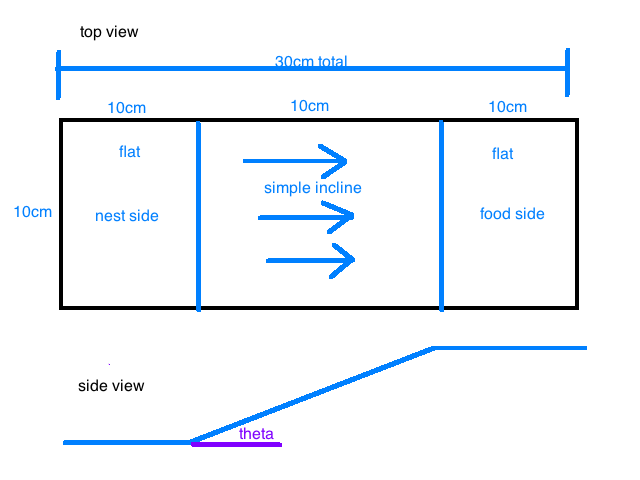
\includegraphics[width=10cm]{simple_incline_schematic}
        \end{figure}
        \item simple hill/crater (whether ``simple
        hill'' or ``simple crater'' depends on angle of incline)
        \begin{figure}[H]
         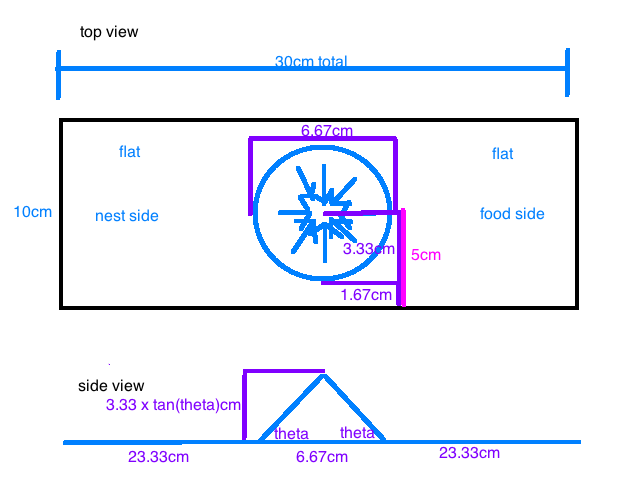
\includegraphics[width=10cm]{simple_hill_schematic}
         \end{figure}
    \end{itemize}
    \item nest/food locations
    \begin{itemize}
    	\item both in center
         \begin{figure}[H]
         	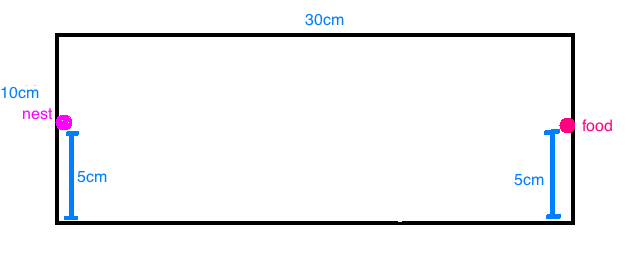
\includegraphics[width=10cm]{middle_food_schematic}
         \end{figure}
        \item in opposite corners
         \begin{figure}[H]
         	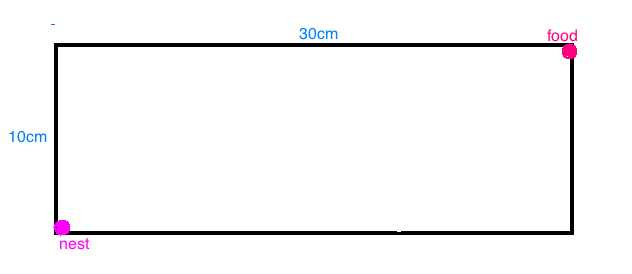
\includegraphics[width=10cm]{cross_food_schematic}
         \end{figure}
    \end{itemize}
    \item angle of incline
    \begin{itemize}
    	\item $\theta = 0, \pm \pi/9, \pm \pi/6, \pm \pi/4, \pm \pi/ 3$ 
    \end{itemize}
    \item vary ants' ``preferred'' heading on incline (assume vertical for all other trials, try these with $\pm \pi/3$ conditions)
    \begin{itemize} 
    	\item vertical
        \item horizontal
        \item 45\degree
        \item no preference
      \end{itemize}
\end{itemize}

Total number of experimental setups (listed from high priority to low priority): 
\begin{itemize}
	\item simple incline/decline with all nest/food locations, all angles of incline, vertical preferred heading
	\[
		1 \times 2 \times 9 \times 1 = 18
	\]
\item simple hill/crater with opposite corners food locations, all angles of incline except 0, vertical preferred heading
	\[
		1 \times 2 \times 8 \times 1 = 16	
	\]
\item all preferred headings with both arena terrains, both nest/food locations, $\pi/6$ and $\pi/3$ angles of incline
	\[
    	4 \times 2 \times 2 \times 2 = 32
    \]
\item TOTAL: 66
	\[
    	18 + 16 + 32 = 66
    \]
\end{itemize}
\end{document}
